\documentclass[tikz, border=2pt]{standalone}
\usepackage{tikz}
\usepackage{pgfplots}
\usetikzlibrary{decorations.pathreplacing,calc}
\begin{document}
    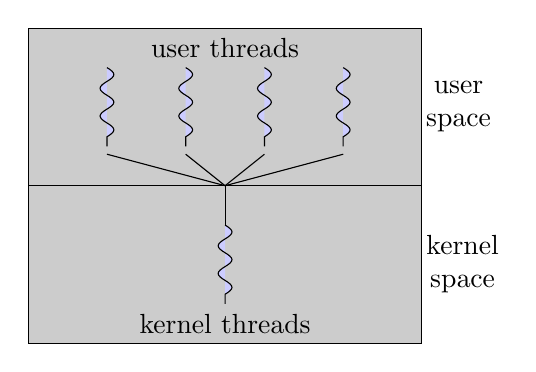
\begin{tikzpicture}
        \draw [fill=black!20] (0,1) rectangle (5,3);
        \draw [fill=black!20] (0,3) rectangle (5,5);
        \foreach \x in {1,...,4}
        {
            \draw[fill=blue!20, decorate, decoration={coil,aspect=0}] (\x,4.5) -- (\x,3.5);
            \draw (\x,3.4) -- (2.5,3);
        }
        \draw (2.5, 3) -- (2.5,2.5);
        \draw[fill=blue!20, decorate, decoration={coil,aspect=0}] (2.5, 2.5) -- (2.5, 1.5);
        \node [above] at (2.5,4.5) {user threads};
        \node [above] at (2.5,1) {kernel threads};
        \node [left, align=center] at (6,4) {user\\space};
        \node [left, align=center] at (6.1,2) {kernel\\space};
    \end{tikzpicture}
\end{document}